%! Author: Henrik Agerholm Ferrari, Þorvaldur Máni Danivalsson, Fei Gu
% This is the EASV CS21 4th Semester IOT Exam project report.
% Group name is
%!TEX encoding = UTF-8 Unicode



% Preamble
\documentclass[a4paper, 12pt]{article}        % here is the document's type which is {article}.
\title{Making a new tomorrow in cyber stalking and e worms}                                   % the title of this document.
\author{Henrik Agerholm Ferrari, Þorvaldur Máni Danivalsson, Fei Gu}
\date{\today}

% Packages
\usepackage{amsmath}
\usepackage{graphicx}
\usepackage{blindtext}
\usepackage[T1]{fontenc}
\usepackage{listings}
\usepackage{xcolor}

\definecolor{codegreen}{rgb}{0,0.6,0}
\definecolor{codegray}{rgb}{0.5,0.5,0.5}
\definecolor{codepurple}{rgb}{0.58,0,0.82}
\definecolor{backcolour}{rgb}{0.95,0.95,0.92}

\lstdefinestyle{mystyle}{
    backgroundcolor=\color{backcolour},
    commentstyle=\color{codegreen},
    keywordstyle=\color{magenta},
    numberstyle=\tiny\color{codegray},
    stringstyle=\color{codepurple},
    basicstyle=\ttfamily\footnotesize,
    breakatwhitespace=false,
    breaklines=true,
    captionpos=b,
    keepspaces=true,
    numbers=left,
    numbersep=5pt,
    showspaces=false,
    showstringspaces=false,
    showtabs=false,
    tabsize=2
}

\lstset{style=mystyle}


% Document
\begin{document}        % the ducument start here

    \maketitle
    \tableofcontents

    \pagebreak
    \section{Problem statement}\label{sec:problem-statement}
    % Which problem for a human is it solving and why is it important

    \paragraph{}
    We want to make a product that can help with the outrageous prices that the security companies charge every
    month for small businesses or private individuals.

    \paragraph{}
    We would be able to make something with Internet of Things,that can trigger sensors and give us some feedback
    to see, if there are any suspicious behaviors going on a certain parameter.

    \paragraph{}
    To fulfill this, we need to:

    \begin{itemize}

        \item Get the modules we need that can be used for the user to easily get access to.

        \item Connect the modules to an ESP32 device, so we can control it over the internet.

        \item Make a program that involves modules that can receive and send feedback.

        \item Set up a database for images to show to the user.

    \end{itemize}

    \section{Illustration of network architecture}\label{sec:illustration-of-network-architecture}
    % Use draw.io make a architecture, remember to name the protocols and the hardwares.
    \subsection{Modules}\label{subsec:modules}

    We decided to use the following modules:

    \begin{itemize}
        \item ESP32-Firebettle * 2
        \item ESP32-Cam
        \item Sound Sensor
        \item PIR Sensor
        \item Buzzer
    \end{itemize}

    \subsection{Net work architecture}\label{subsec:net-work-architecture}

    \begin{figure}[h]
        \centering
        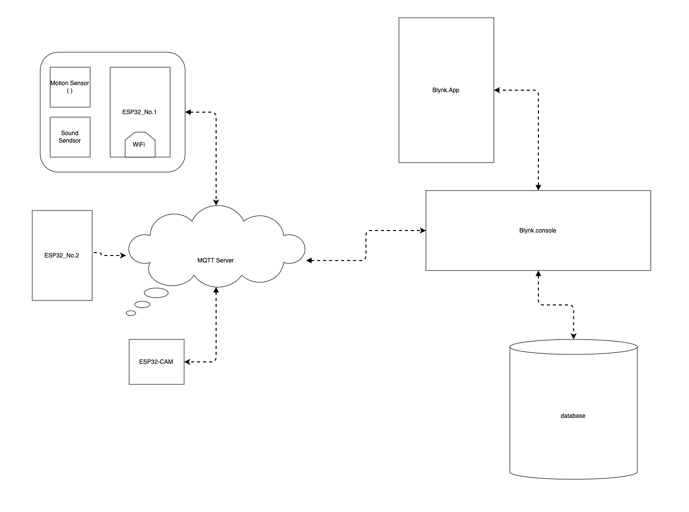
\includegraphics[width=1\textwidth]{CircuitLayOut/img}
        \caption{net work architecture}
        \label{fig:figure1}
    \end{figure}

    \paragraph{}
    Following the problem statement, we have to design the architecture base on three different device using three ESP32 MCU\@.
    And make sure all those device can communicate to each other to transport the data.
    And we should have a front-end mobile application to control the device and get to view the data.
    Afterward, we need a storage to contain the footage of the camera shoot.

    \paragraph{}
    Because the real situation which is the most app on the mobile device to be use fully function should be paid.
    And this is an academic porject that we should not to pay. So we decide to use the free version of Blynk as the
    mobile app UI. And in case we need use firebase web app to show the footage.

    \paragraph{}
    The MQTT server will subscribe the topic
    \pagebreak
    \section{Illustration of the hardware setup}\label{sec:illustration-of-the-hardware-setup}
    % Use fritzing or just use circuiTikZ make the circuit layout\pm
    \paragraph{}
    This part will explain the circuit and wire connection.

    \blindtext{}


    \pagebreak
    \subsection{esp32No1 Sensor}\label{subsec:esp32no1-sensor}
    \paragraph{}
    This is the part ESP32 to connect to the sensors.

    \blindtext{}



    \begin{figure}[h]
        \caption{ESP32 no.1 connect to sensors}
        \centering
        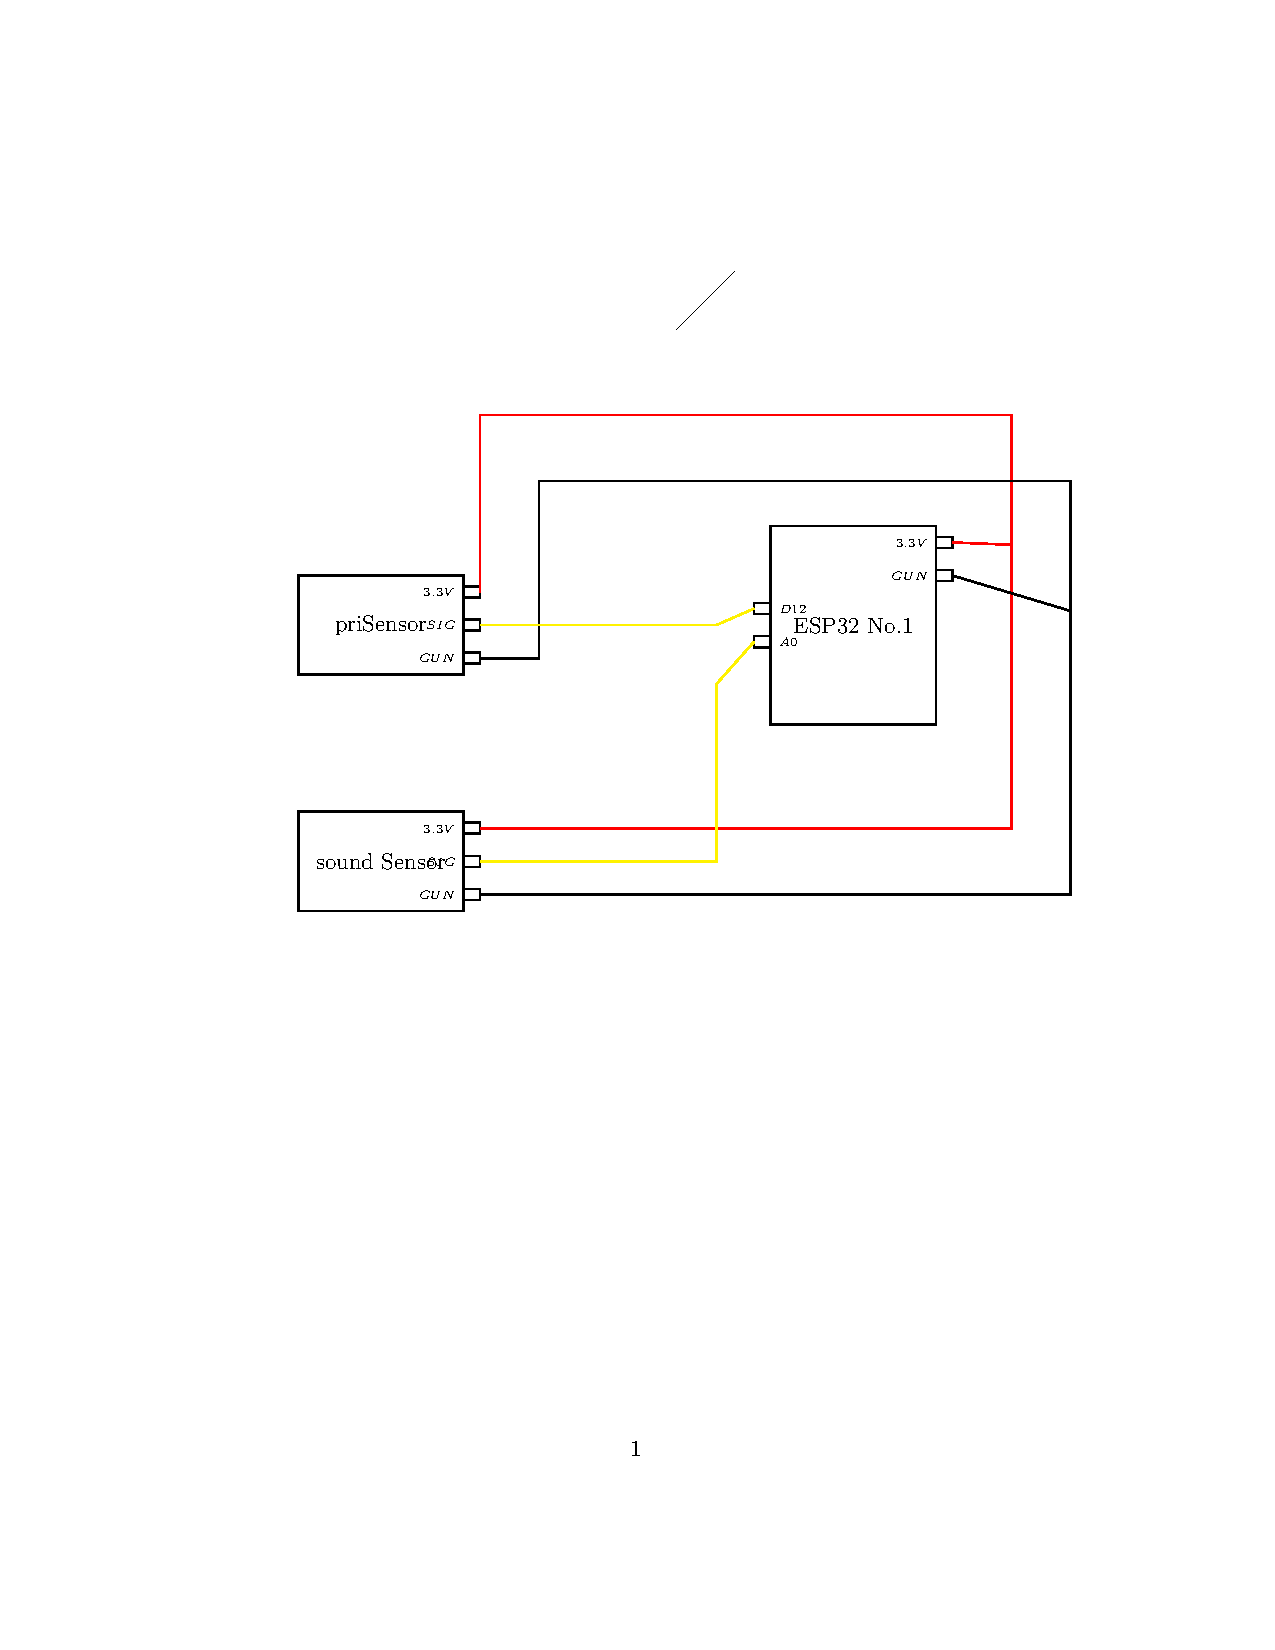
\includegraphics[width=0.5\textwidth]{../out/ESP32_No1_connect_Sensor}
        \label{fig:figure2}
    \end{figure}


    \pagebreak
    \subsection{esp32No2 Buzzer}\label{subsec:esp32no2-buzzer}
    \paragraph{}
    This part is talking about the ESP32 connect to the buzzer.
    this is a quite simple circuit we connect the 3.3 to power and gun to gun.
    and then connect the sig pin to D12 to set the data trans.

    \blindtext{}



    \begin{figure}[h]
        \caption{ESP32 no.2 connect to buzzer and LED-display}\label{fig:figure3}
        \centering
        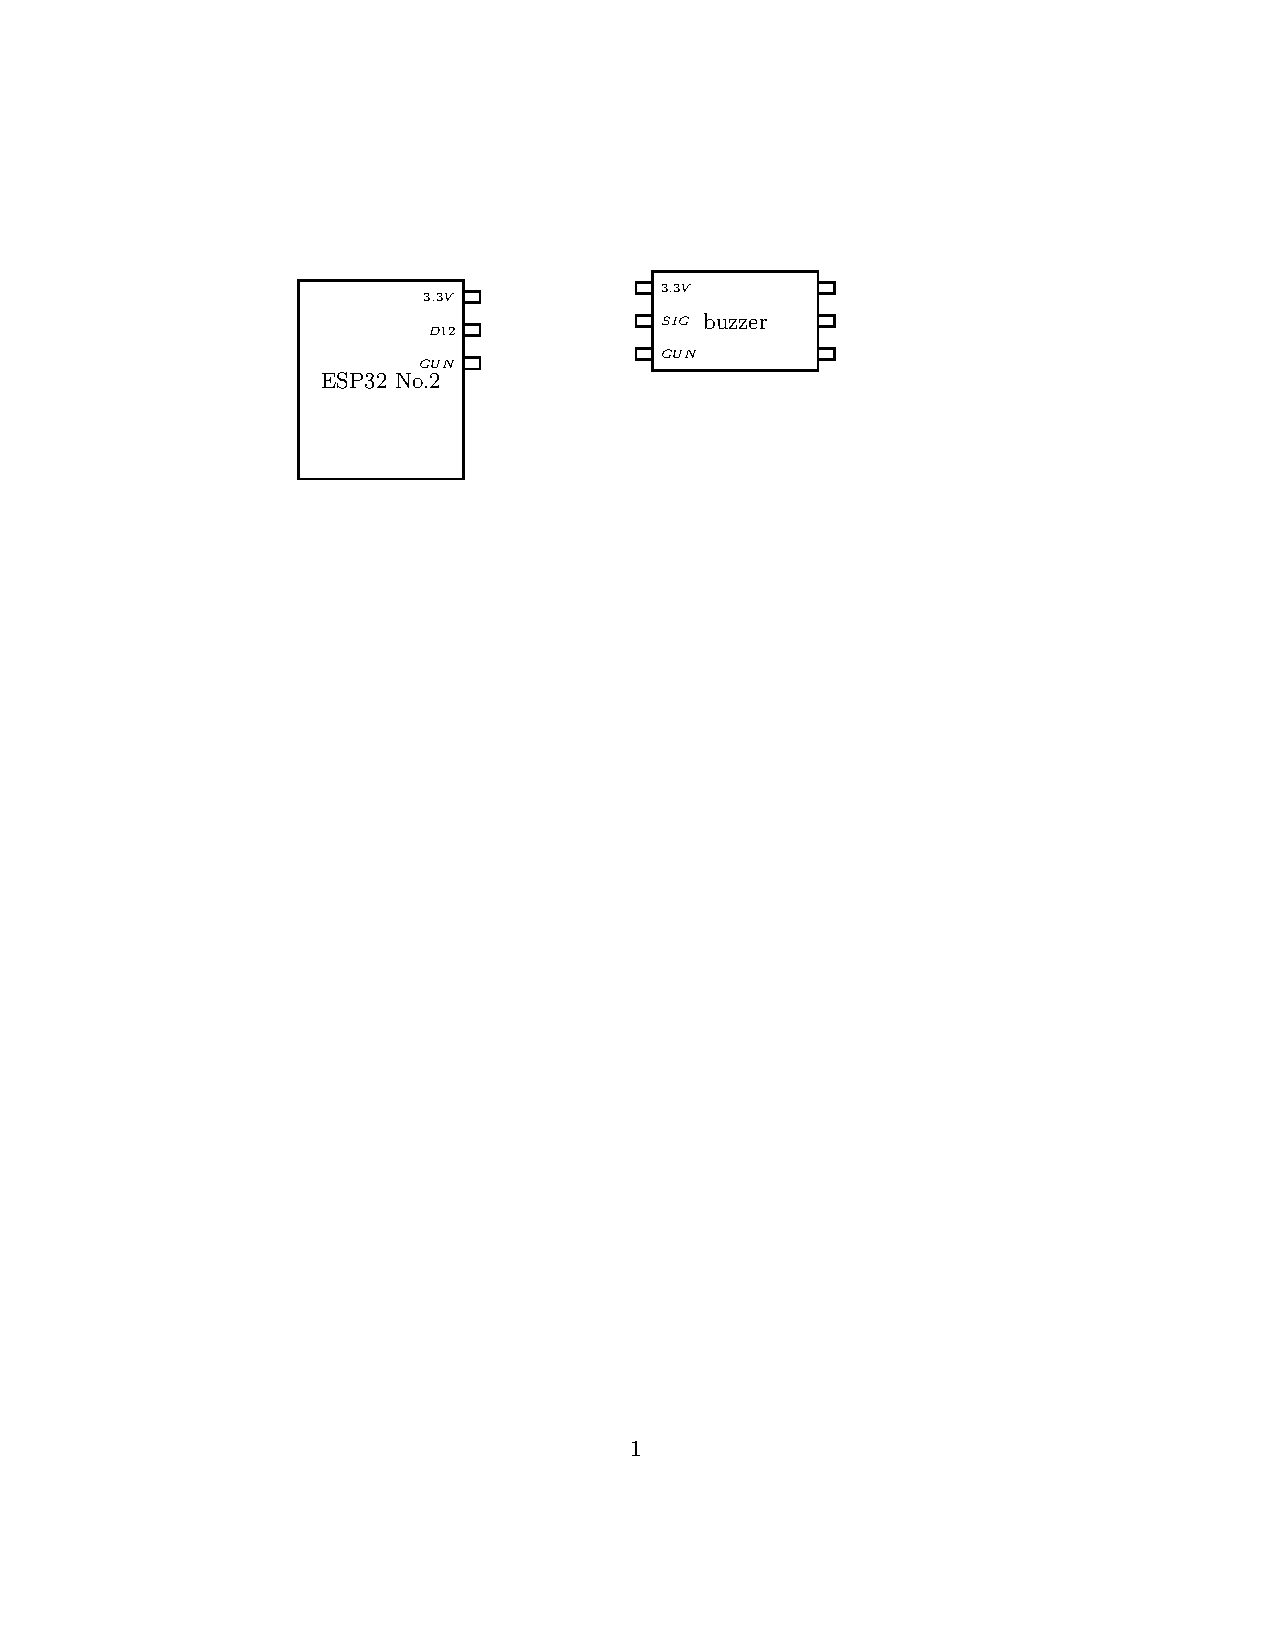
\includegraphics[width=0.5\textwidth]{../out/ESP32_No.2_connect_Buzzer}
    \end{figure}

    \pagebreak
    \subsection{esp32Cam}\label{subsec:esp32cam}
    \paragraph{}
    This part is the connection about the Esp32 Camera can be flash under the develop mode.
    And when we leave the development mode then just unplug all the wires except the power and ground.

    \blindtext{}

    \begin{figure}[h]
        \caption{ESP32 CAM}\label{fig:figure4}
        \centering
        \includegraphics[width=0.5\textwidth]{../out/ESP32Cam_connect_TypeCAdapter}
    \end{figure}

    \pagebreak
    \section{Conclusion}\label{sec:conclusion}

    \paragraph{}
    We ended up with a rough prototype that can be used for a security system.

    \paragraph{}
    We really wanted to show live feed from the ESP32-Camera, but all services that could help us with this costs money to use.
    That is why we used Blynk for some feedback from some modules because we thought that the cam service was free,
    but unfortunately it was not.

    \paragragh{}
    It was just a nice and easy way for the user to get notified if something
    was in motion on their mobile phone.

    \pagebreak
    \appendix

    \section{ESP32-Sensor Code}
    \lstinputlisting[language=C++]{../../3.ArduinoProject/examProject_ESP32_No1_Sensor/src/main.cpp}
    \pagebreak

    \section{ESP32-Buzzer Code}
    \lstinputlisting[language=C++]{../../3.ArduinoProject/examProject_ESP32_No2_buzzer/src/main.cpp}
    \pagebreak

    \section{ESP32-Cam Code}
    \lstinputlisting[language=C++]{../../3.ArduinoProject/esamProject_ESP32_CAM/src/main.cpp}
    \pagebreak



\end{document}
